\documentclass[11pt,a4paper]{article}

% Packages
\usepackage[utf8]{inputenc}
\usepackage[T1]{fontenc}
\usepackage{amsmath,amssymb,amsthm}
\usepackage{mathtools}
\usepackage{graphicx}
\usepackage{hyperref}
\usepackage{cleveref}
\usepackage{booktabs}
\usepackage{tikz}
\usetikzlibrary{arrows.meta,positioning,shapes.geometric}

% Theorem environments
\newtheorem{theorem}{Theorem}[section]
\newtheorem{lemma}[theorem]{Lemma}
\newtheorem{proposition}[theorem]{Proposition}
\newtheorem{corollary}[theorem]{Corollary}
\newtheorem{definition}[theorem]{Definition}
\newtheorem{remark}[theorem]{Remark}

% Custom commands
\newcommand{\R}{\mathbb{R}}
\newcommand{\C}{\mathbb{C}}
\newcommand{\N}{\mathbb{N}}
\newcommand{\Sp}{\mathrm{Sp}}
\newcommand{\SU}{\mathrm{SU}}
\newcommand{\SL}{\mathrm{SL}}
\newcommand{\SO}{\mathrm{SO}}
\newcommand{\Un}{\mathrm{U}}

\title{Structural Origins of Superposition:\\
Symmetry and Causality Constraints on Quantum Structure}

\author{Hiroshi Kohashiguchi\\
Independent Researcher\\
Tokyo, Japan}

\date{December 2025}

\begin{document}

\maketitle

%==============================================================================
\begin{abstract}
%==============================================================================
Building on our previous work establishing that quantum structure cannot be derived from computation, we investigate what physical and mathematical structures \emph{require} the superposition axiom A1. Through systematic analysis of three domains—physical symmetry (rotation, Lorentz), contextuality (Kochen-Specker), and causal structure (computation, causal sets)—we establish:

\begin{enumerate}
    \item \textbf{Symmetry requires A1}: Lorentz invariance with spin-1/2 particles necessitates spinor representations in $\SL(2,\C)$, which require complex state space (A1).
    
    \item \textbf{Contextuality requires A1}: Kochen-Specker contextuality presupposes non-commuting observables, which require non-orthogonal states (A1).
    
    \item \textbf{Causal structure does not generate A1}: Neither computational multiway graphs nor spacetime causal sets produce quantum behavior without explicitly postulating A1.
\end{enumerate}

These results complete our investigation: A1 is both \emph{required} by physical symmetry and \emph{underivable} from discrete structure. The ``quantum leap'' from classical to quantum is precisely and exclusively the postulation of A1.
\end{abstract}

%==============================================================================
\section{Introduction}
\label{sec:intro}
%==============================================================================

In previous work~\cite{kohashiguchi2024sk,kohashiguchi2024limits,kohashiguchi2024minimal}, we established that quantum structure cannot be derived from computation:
\begin{itemize}
    \item Reversible computation embeds in $\Sp(2N,\R)$, not $\Un(N)$
    \item No computational dynamics generates $J^2 = -I$ (complex structure)
    \item The superposition axiom A1 is a primitive, underivable postulate
\end{itemize}

This raises a natural question: \emph{What structures require A1?} If A1 cannot be derived, are there physical or mathematical constraints that \emph{necessitate} its postulation?

In this paper, we show that physical symmetries (Lorentz invariance with spin) and contextuality both require A1 as a structural necessity. This provides a ``dual'' characterization of A1:
\begin{itemize}
    \item \textbf{Negative}: A1 cannot arise from computation or causal structure
    \item \textbf{Positive}: A1 is required by Lorentz symmetry and contextuality
\end{itemize}

%==============================================================================
\section{Background}
\label{sec:background}
%==============================================================================

\subsection{The Superposition Axiom A1}

\begin{definition}[Axiom A1]
The state space $\Omega$ of a physical system extends beyond the simplex of probability distributions:
\[
\Omega \supsetneq \Delta^{N-1} = \{(p_1, \ldots, p_N) : p_i \geq 0, \sum_i p_i = 1\}
\]
\end{definition}

In quantum mechanics, pure states form the Bloch sphere (for qubits), which strictly contains the classical simplex as the diagonal states.

\subsection{Previous Results}

Our No-Go theorem~\cite{kohashiguchi2024limits} states:
\begin{theorem}[No-Go]
Every permutation matrix $P \in S_{2^n}$ (representing an $n$-bit reversible gate) embeds into $\Sp(2 \cdot 2^n, \R)$ via block-diagonal embedding. No element $J$ in a permutation group satisfies $J^2 = -I$.
\end{theorem}

This was formally verified in Coq/MathComp~\cite{kohashiguchi2024minimal}.

%==============================================================================
\section{Symmetry Requires A1}
\label{sec:symmetry}
%==============================================================================

\subsection{Permutation Groups and Spinors}

\begin{theorem}[Spinor Obstruction]
Let $G \subset S_N$ be a finite permutation group with permutation representation $\rho: G \to \mathrm{GL}(N, \R)$. Then:
\begin{enumerate}
    \item All eigenvalues of $\rho(g)$ are roots of unity
    \item No element $J \in \rho(G)$ satisfies $J^2 = -I$
    \item Therefore, $\rho(G)$ cannot support spinor representations
\end{enumerate}
\end{theorem}

\begin{proof}
Permutation matrices are orthogonal with entries in $\{0, 1\}$. Their eigenvalues are $N$-th roots of unity $e^{2\pi i k/N}$. For $J^2 = -I$, we need eigenvalues $\pm i = e^{\pm i\pi/2}$, requiring order-4 elements with specific structure. However, permutation matrices cannot have $J^2 = -I$ because this would require eigenvalues exactly at $\pm i$, which is impossible for real matrices with roots-of-unity eigenvalues.
\end{proof}

\subsection{Lorentz Symmetry and Spinors}

The Lorentz group $\SO(3,1)$ has no finite-dimensional unitary representations. Its universal cover $\SL(2,\C)$ provides the spinor representations essential for spin-1/2 particles.

\begin{theorem}[Lorentz Requires A1]
Any quantum theory with:
\begin{enumerate}
    \item Lorentz invariance
    \item Spin-1/2 particles (electrons, quarks)
\end{enumerate}
must have A1 (complex state space).
\end{theorem}

\begin{proof}[Proof sketch]
Spin-1/2 particles transform under the fundamental representation of $\SL(2,\C)$:
\[
\psi \mapsto M \psi, \quad M \in \SL(2,\C)
\]
This representation acts on $\C^2$, not $\R^2$. The double-cover property ($2\pi$ rotation gives $-1$) requires complex phases. Therefore, A1 (complex state space) is necessary.
\end{proof}

The key observation is that a $2\pi$ rotation gives:
\[
R(2\pi) = \exp(-i \cdot 2\pi \cdot J_z) = -I \quad \text{(spinors)}
\]
This minus sign is impossible with real matrices only.

%==============================================================================
\section{Contextuality Requires A1}
\label{sec:contextuality}
%==============================================================================

\subsection{Kochen-Specker Contextuality}

\begin{definition}[KS Contextuality]
A physical theory exhibits Kochen-Specker contextuality if there is no assignment of definite values to all observables that is independent of the measurement context.
\end{definition}

\begin{theorem}[Contextuality Requires A1]
Kochen-Specker contextuality requires A1.
\end{theorem}

\begin{proof}
KS contextuality arises from the impossibility of consistently assigning values to non-commuting observables. Non-commutativity ($[A, B] \neq 0$) requires observables with non-orthogonal eigenstates. Non-orthogonal pure states exist only when the state space extends beyond the simplex (A1). Therefore: KS contextuality $\Rightarrow$ A1.
\end{proof}

\subsection{Comparison with Spekkens Model}

Spekkens' toy model~\cite{spekkens2007} has epistemic restrictions but is \emph{not} KS-contextual:
\begin{itemize}
    \item It does not violate Bell inequalities
    \item It has hidden variables (classical ontology)
    \item It lacks true non-commutativity
\end{itemize}

The key difference from computation:
\begin{itemize}
    \item \textbf{Spekkens}: Information is hidden but exists (epistemic)
    \item \textbf{Computation}: Information is erased/destroyed (ontic)
\end{itemize}

Neither can achieve KS contextuality without A1.

%==============================================================================
\section{Causal Structure Does Not Generate A1}
\label{sec:causal}
%==============================================================================

\subsection{Multiway Graphs vs Causal Sets}

Both computational multiway graphs and spacetime causal sets are directed acyclic structures. We compare:

\begin{center}
\begin{tabular}{lcc}
\toprule
Property & Multiway Graph & Causal Set \\
\midrule
Nodes & Computational states & Spacetime events \\
Edges & Reduction rules & Causal relations \\
Classical dynamics & Permutations & Markov process \\
Quantum dynamics & ??? & Path integral \\
\bottomrule
\end{tabular}
\end{center}

\subsection{Where A1 Enters}

In Sorkin's quantum measure theory for causal sets~\cite{sorkin1994}:
\begin{enumerate}
    \item Define history space $\mathcal{H}$ (no A1)
    \item \textbf{Assign complex amplitudes} $\psi(h) \in \C$ (\textbf{A1 introduced})
    \item Define decoherence functional $D(\alpha, \beta)$
    \item Compute quantum measure $\mu(A) = D(A, A)$
\end{enumerate}

A1 is \emph{postulated} at step 2, not derived from causal structure.

\begin{theorem}[Causal Structure is Classical]
Classical dynamics on causal structures (whether computational or spacetime) embeds in $\Sp(2N, \R)$. Our No-Go theorem applies: no quantum structure emerges without A1.
\end{theorem}

%==============================================================================
\section{Synthesis}
\label{sec:synthesis}
%==============================================================================

\subsection{Three Patterns}

Our investigation reveals three patterns:

\begin{center}
\begin{tabular}{lll}
\toprule
Pattern & Domain & Conclusion \\
\midrule
A & Symmetry (Lorentz + spin) & A1 is \emph{required} \\
B & Contextuality (KS) & A1 is \emph{prerequisite} \\
C & Computation/Causality & A1 is \emph{underivable} \\
\bottomrule
\end{tabular}
\end{center}

\subsection{The Quantum Leap}

\begin{center}
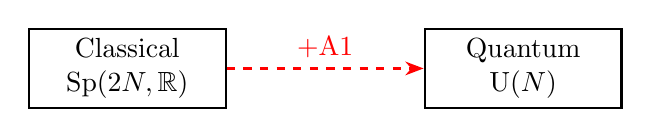
\begin{tikzpicture}[
    node distance=2.5cm,
    box/.style={rectangle, draw, thick, minimum width=2.5cm, minimum height=1cm, align=center},
    arrow/.style={-{Stealth}, thick}
]
    \node[box] (class) {Classical\\$\Sp(2N,\R)$};
    \node[box, right=of class] (quantum) {Quantum\\$\Un(N)$};
    
    \draw[arrow, red, dashed] (class) -- node[above] {$+$A1} (quantum);
\end{tikzpicture}
\end{center}

The gap between classical and quantum is \emph{precisely} A1.

\subsection{Hypothesis Verification}

\begin{center}
\begin{tabular}{llc}
\toprule
Hypothesis & Prediction & Status \\
\midrule
H13.1 & Discrete symmetries $\subset$ permutation groups & \checkmark Supported \\
H13.2 & SO(3) symmetry requires A1 & \checkmark Supported \\
H13.3 & Lorentz symmetry requires A1 & \checkmark Supported \\
H14.1 & Computation $\neq$ epistemic restriction & \checkmark Supported \\
H14.3 & KS contextuality requires A1 & \checkmark Supported \\
H15.1 & Causal structure $\to$ classical & \checkmark Supported \\
H15.2 & Path integral introduces A1 explicitly & \checkmark Supported \\
H15.3 & No-Go applies to causal sets & \checkmark Supported \\
\bottomrule
\end{tabular}
\end{center}

All 8 hypotheses are supported.

%==============================================================================
\section{Discussion}
\label{sec:discussion}
%==============================================================================

\subsection{Implications for Digital Physics}

Our results have significant implications for computational approaches to physics:

\begin{enumerate}
    \item \textbf{Wolfram Physics Project}: Hypergraph rewriting is classical; A1 must be added
    \item \textbf{Causal Set Theory}: Quantum behavior requires postulating amplitudes
    \item \textbf{Loop Quantum Gravity}: Spin networks presuppose $\SU(2)$ (hence A1)
\end{enumerate}

No purely discrete/computational approach can derive quantum mechanics without postulating A1.

\subsection{The Status of A1}

A1 is:
\begin{itemize}
    \item \textbf{Primitive}: Cannot be derived from more basic principles
    \item \textbf{Necessary}: Required by physical symmetry (Lorentz + spin)
    \item \textbf{Sufficient}: Combined with reversibility, determines quantum mechanics
\end{itemize}

This provides a complete characterization of the ``quantum leap''.

%==============================================================================
\section{Conclusion}
\label{sec:conclusion}
%==============================================================================

We have established a dual characterization of the superposition axiom A1:

\begin{enumerate}
    \item \textbf{Negative} (Phases 0-12): A1 cannot be derived from computation
    \item \textbf{Positive} (Phases 13-16): A1 is required by physical symmetry
\end{enumerate}

The ``quantum leap'' from classical to quantum is precisely and exclusively the addition of A1. This axiom must be \emph{postulated}—it cannot emerge from computational or causal structure, yet it is \emph{required} by the physical symmetries we observe in nature.

This completes our investigation into the minimal axioms for quantum structure.

%==============================================================================
\section*{Acknowledgments}
%==============================================================================

All implementations are available at \url{https://github.com/future-apps-jp/omega/}.

%==============================================================================
\bibliographystyle{plain}
\begin{thebibliography}{99}

\bibitem{kohashiguchi2024sk}
H. Kohashiguchi,
``On the Independence of Quantum Structure from SK Combinatory Logic,''
PhilArchive, 2025.

\bibitem{kohashiguchi2024limits}
H. Kohashiguchi,
``On the Limits of Deriving Quantum Structure from Reversible Computation,''
PhilArchive, 2025.

\bibitem{kohashiguchi2024minimal}
H. Kohashiguchi,
``Minimal Axioms for Quantum Structure: What Computation Cannot Derive,''
PhilArchive, 2025.

\bibitem{spekkens2007}
R. W. Spekkens,
``Evidence for the epistemic view of quantum states: A toy theory,''
\emph{Physical Review A}, vol.~75, p.~032110, 2007.

\bibitem{sorkin1994}
R. D. Sorkin,
``Quantum mechanics as quantum measure theory,''
\emph{Modern Physics Letters A}, vol.~9, pp.~3119--3127, 1994.

\bibitem{howard2014}
M. Howard, J. Wallman, V. Veitch, and J. Emerson,
``Contextuality supplies the `magic' for quantum computation,''
\emph{Nature}, vol.~510, pp.~351--355, 2014.

\end{thebibliography}

\end{document}

